% Lecture Template for ME3001-001-Tristan Hill - Spring 2017 - Fall 2017
% 
% Mechanical Engineering Analysis with MATLAB
%
% Introduction to Analysis

% Document settings
\documentclass[11pt]{article}
\usepackage[margin=1in]{geometry}
\usepackage[pdftex]{graphicx}
\usepackage{multirow}
\usepackage{setspace}
\usepackage{hyperref}
\usepackage{color,soul}
\usepackage{fancyvrb}
\usepackage{framed}
%\usepackage{wasysym}
\usepackage{multicol}
\usepackage{ amssymb }
\usepackage{amsmath}



\pagestyle{plain}
\setlength\parindent{0pt}
\hypersetup{
    bookmarks=true,         % show bookmarks bar?
    unicode=false,          % non-Latin characters in Acrobat’s bookmarks
    pdftoolbar=true,        % show Acrobat’s toolbar?
    pdfmenubar=true,        % show Acrobat’s menu?
    pdffitwindow=false,     % window fit to page when opened
    pdfstartview={FitH},    % fits the width of the page to the window
    pdftitle={My title},    % title
    pdfauthor={Author},     % author
    pdfsubject={Subject},   % subject of the document
    pdfcreator={Creator},   % creator of the document
    pdfproducer={Producer}, % producer of the document
    pdfkeywords={keyword1} {key2} {key3}, % list of keywords
    pdfnewwindow=true,      % links in new window
    colorlinks=true,       % false: boxed links; true: colored links
    linkcolor=red,          % color of internal links (change box color with linkbordercolor)
    citecolor=green,        % color of links to bibliography
    filecolor=magenta,      % color of file links
    urlcolor=blue           % color of external links
}

% assignment number 
\newcommand{\NUM}{1 } 
\newcommand{\VSpaceSize}{2mm} 
\newcommand{\HSpaceSize}{2mm} 

\newcommand{\Lagr}{\mathcal{L}}

\definecolor{mygray}{rgb}{.6, .6, .6}

\setulcolor{red} 
\setstcolor{green} 
\sethlcolor{mygray} 

\begin{document}

\textbf{ \LARGE ME 3050 Lecture - Dynamic Modeling and Controls} \vspace{3mm}\\
\textbf{ \hspace*{5mm}Tristan W. Hill - Tennessee Technological University - Spring 2020 } \vspace{3mm}\\


\textbf{ \LARGE Ch. 8 - System Response in the Time Domain} \\

\begin{itemize}


\item \textbf{ \LARGE (8.1) Time Response of 1$^{st}$ Order Systems} \\

\begin{itemize}


\item \textbf{ \Large Consider the model of the moving mass we derived.}\\

			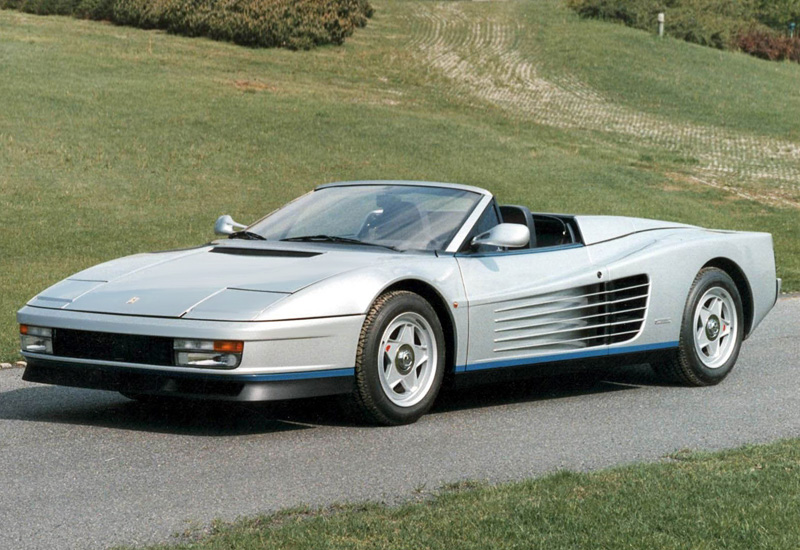
\includegraphics[scale=.25]{ferrari.jpg} \\

\item \textbf{ \Large The EOM is:}\\

	\scalebox{1.5}{$m\dot{v} +cv=0$} \\

\item \textbf{ \Large Solve for $v(t)$ using a method of your choice. \\\\ }\\

\item \textbf{\large The method of Laplace Transforms is shown.}\\\\

	\scalebox{1.5}{$\Lagr{\{m\dot{v} +cv}=0\}$ $ \implies$  $m [sV(s) -v(0) ] +cV(s)=0$} \\

	\scalebox{1.5}{$(ms+c)V(s)=\frac{mv(0)}{(ms+c)} = \frac{V(0)}{s+\frac{c}{m}}$}\\\\

\item \textbf{\large We can find the expected result from the table.}\\\\

	\scalebox{1.5}{$v(t)=v(0)e^{-\frac{c}{m}t} = v(0)e^{-\frac{t}{\tau}} $ \hspace{5mm} with \hspace{5mm}$\tau = $}\\



	\newpage
\item \textbf{ \Large Sketch the System Response in the time Domain.}

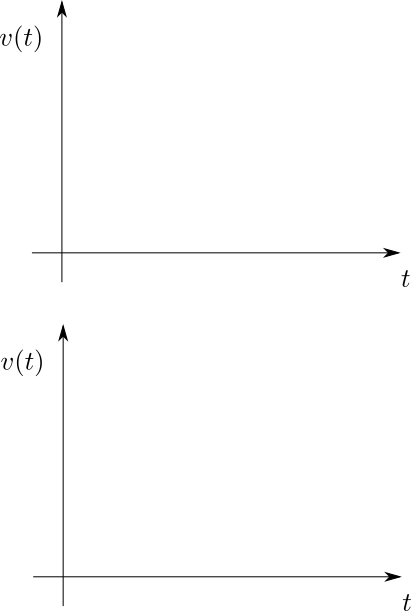
\includegraphics[scale=1]{lecture1_fig1.png} \\

\item \textbf{\large Is this a stable system? What does that even mean?}\\\\


\end{itemize}
		

	\newpage
\item \textbf{ \Large Consider the model subject to a Step Input, $f(t)$.}\\
\begin{multicols}{2}
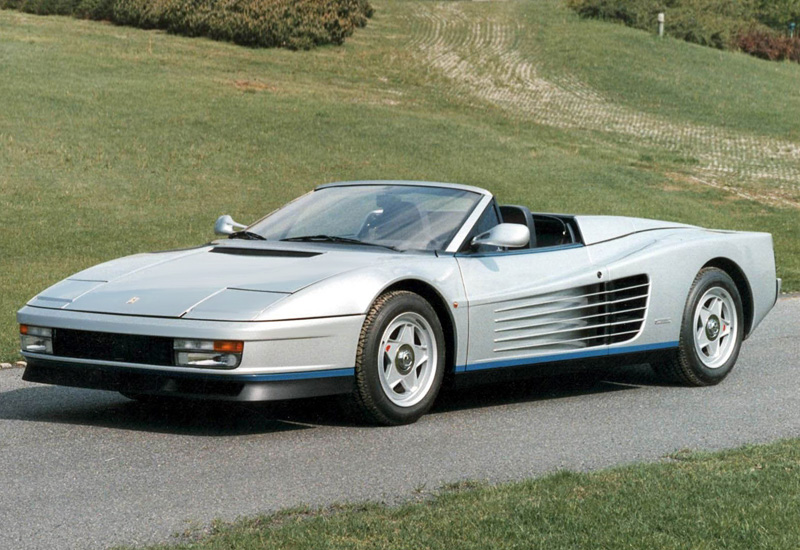
\includegraphics[scale=.25]{ferrari.jpg}  

\scalebox{1.5}{$m\dot{v} +cv=f(t)$} \\\\

\[f(t) = \begin{cases} 
      0 & t < 0 \\
      F & t\geq 0 \\
   \end{cases}
\]\\

\end{multicols}

\item \textbf{\large The method of Laplace Transforms is shown.}\\\\

	\scalebox{1.5}{$\Lagr{\{m\dot{v} +cv}=F\}$ $ \implies$  $m [sV(s) -v(0) ] +cV(s)=\frac{F}{c}$} \\\\

	\scalebox{1.5}{$(ms+c)V(s)=\frac{F}{s}+mv(0)$} \\

\item \textbf{\large Partial Fraction Expansion leads to the following form.}\\\\

	\scalebox{1.5}{$V(s)=\frac{F}{s(ms+c)}+\frac{mv(0)}{ms+c}\implies \frac{F}{s(ms+c)}=\frac{a}{s} +\frac{b}{ms+c}$} \\

\item \textbf{\large 'Cover up' to find the coefficients.}\\\\

	\scalebox{1.5}{$a=\frac{F}{m\times0+c} $ \hspace{5mm} and \hspace{5mm} $b=\frac{F}{\frac{-c}{m}}=\frac{-Fm}{c}$}

\item \textbf{\large This leads to a form that can be inverted with the table.}\\

\scalebox{1.5}{$V(s)=\frac{F}{c}\{ \frac{1}{s}-\frac{1}{s+\frac{c}{m}}\}+\frac{v(0)}{s+\frac{c}{m}}$} \\\\

\scalebox{1.5}{$v(t)=\frac{F}{C}\{1-e^{-\frac{t}{\tau}} \} + v(0)e^{-\frac{t}{\tau}} = \{v(0)-\frac{F}{c}\}e^{-\frac{t}{\tau}} + \frac{F}{c}$  }

\newpage

\item \textbf{\large In these forms we can see the different components of the response.}\\

\scalebox{1.5}{$v(t)=\frac{F}{C}\{1-e^{-\frac{t}{\tau}} \} + v(0)e^{-\frac{t}{\tau}} = \{v(0)-\frac{F}{c}\}e^{-\frac{t}{\tau}} + \frac{F}{c}$  } \vspace{20mm}\\


\Large
\begin{itemize}

\item Forced Response\\

\item Free Response\\

\item Transient Response\\

\item Steady-State Response

\end{itemize}



	\newpage
\item \textbf{ \Large Sketch the System Response in the time Domain.}

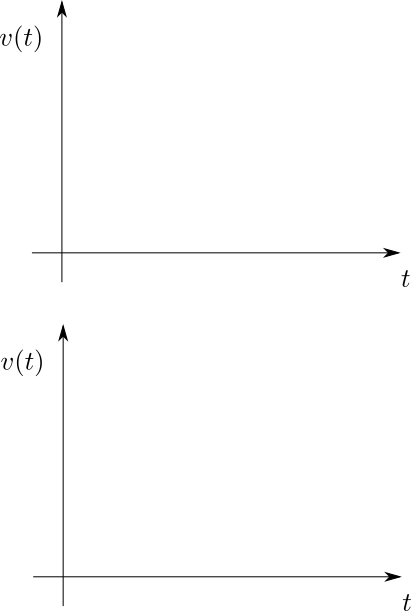
\includegraphics[scale=1]{lecture1_fig1.png} \\
	\end{itemize}

\end{document}



